\documentclass[compress, aspectratio=169]{beamer}

%presentation layout

\mode<presentation>
{
  \usetheme{Berlin}
  % \usecolortheme{dove}
  \setbeamercolor{structure}{bg=white,fg=black}
  \setbeamercolor{normal text}{bg=white,fg=black}
  \setbeamercolor{titlepage}{bg=white,fg=black}
  \setbeamercolor{titlelike}{bg=white,fg=black}
  \setbeamercolor{palette primary}{bg=white}
  \setbeamercolor{palette secondary}{bg=gray, fg=white}
  \setbeamercolor{palette tertiary}{bg=gray, fg=white}
  \setbeamercolor{palette quarternary}{bg=white}
  \setbeamercovered{transparent}
  \useinnertheme{rectangles}
  %\usefonttheme{serif}
}

\setbeamertemplate{navigation symbols}{}

%loading packages
\usepackage[ngerman]{babel}
\usepackage[T1]{fontenc}
\usepackage[utf8]{inputenc}
\usepackage{graphicx}
\usepackage{amsmath}
\usepackage{framed}
\usepackage{caption}
\usepackage{subcaption}
\usepackage{multicol}

% vorgeplaenkel
\title[StAPf-Bericht]{StAPF-Bericht}

\author{Ständiger Ausschuss aller Physikfachschaften}

\institute[Zusammenkunft aller Physikfachschaften]

\date{12. Mai 2021}

\subject{Bericht des StAPF}

\begin{document}

\begin{frame}[plain]{}
  \titlepage
\end{frame}


\section{StAPF}

\begin{frame}
\centering
\Huge Berichte der ZaPF-Gremien
\end{frame}


\begin{frame}{Gewählte Mitglieder im StAPF}

  \begin{minipage}{.28\textwidth}
    \begin{figure}
      \begin{minipage}[c]{.57\textwidth}
        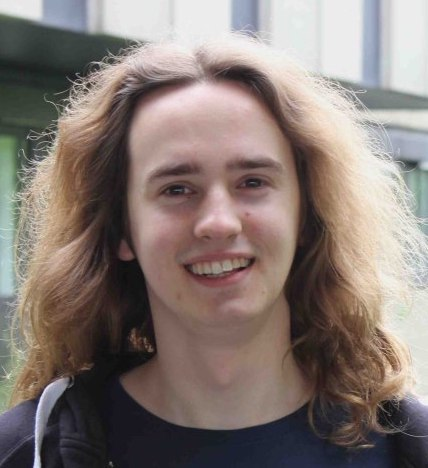
\includegraphics[draft, height=0.3\textheight]{andy.jpg}
      \end{minipage} \hfill
      \begin{minipage}[c]{.4\textwidth}
        \caption*{Andreas Drotloff\\Uni Würzburg}
      \end{minipage}
    \end{figure}
  \end{minipage}
\hfill
  \begin{minipage}{.28\textwidth}
    \begin{figure}
      \begin{minipage}[c]{.5\textwidth}
        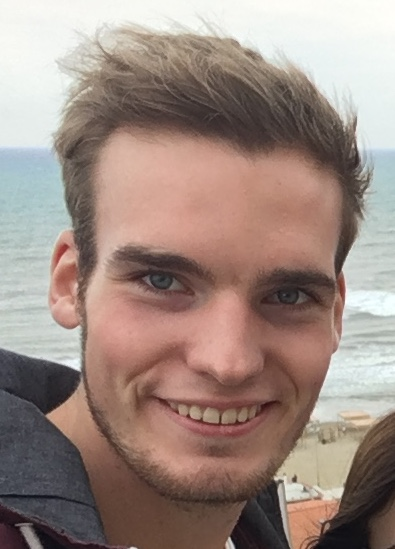
\includegraphics[draft, height=0.35\textheight]{chris.jpeg}
      \end{minipage} \hfill
      \begin{minipage}[c]{.47\textwidth}
        \caption*{Christoph Blattgerste\\Uni Heidelberg}
      \end{minipage}
    \end{figure}
  \end{minipage}
  \hfill
  \begin{minipage}{.28\textwidth}
    \begin{figure}
      \begin{minipage}[r]{.57\textwidth}
        
\includegraphics[draft, height=0.3\textheight]{leon.jpg}
      \end{minipage} \hfill
      \begin{minipage}[c]{.4\textwidth}
        \caption*{Leon Nutzinger \\FU Berlin}
      \end{minipage}
    \end{figure}
  \end{minipage}

  \vspace{1cm}
  \hspace{0.1\textwidth}
   \begin{minipage}{.28\textwidth}
    \begin{figure}
      \begin{minipage}[c]{.57\textwidth}
        \includegraphics[draft, height=0.35\textheight]{anna.jpeg}
      \end{minipage} \hfill
      \begin{minipage}[c]{.4\textwidth}
        \caption*{Sophie Pengers \\Uni Köln}
      \end{minipage}
    \end{figure}
  \end{minipage}
  \hspace{0.1\textwidth}
  \begin{minipage}{.28\textwidth}
    \begin{figure}
      \begin{minipage}[c]{.57\textwidth}
        \includegraphics[draft, height=0.35\textheight]{vicky.jpg}
      \end{minipage} \hfill
      \begin{minipage}[c]{.4\textwidth}
        \caption*{Maximilian Schneider \\Uni Würzburg}
      \end{minipage}
    \end{figure}
  \end{minipage}
  \hspace{0.1\textwidth}

\end{frame}

% \begin{minipage}{.5\textwidth}
% \centering
% 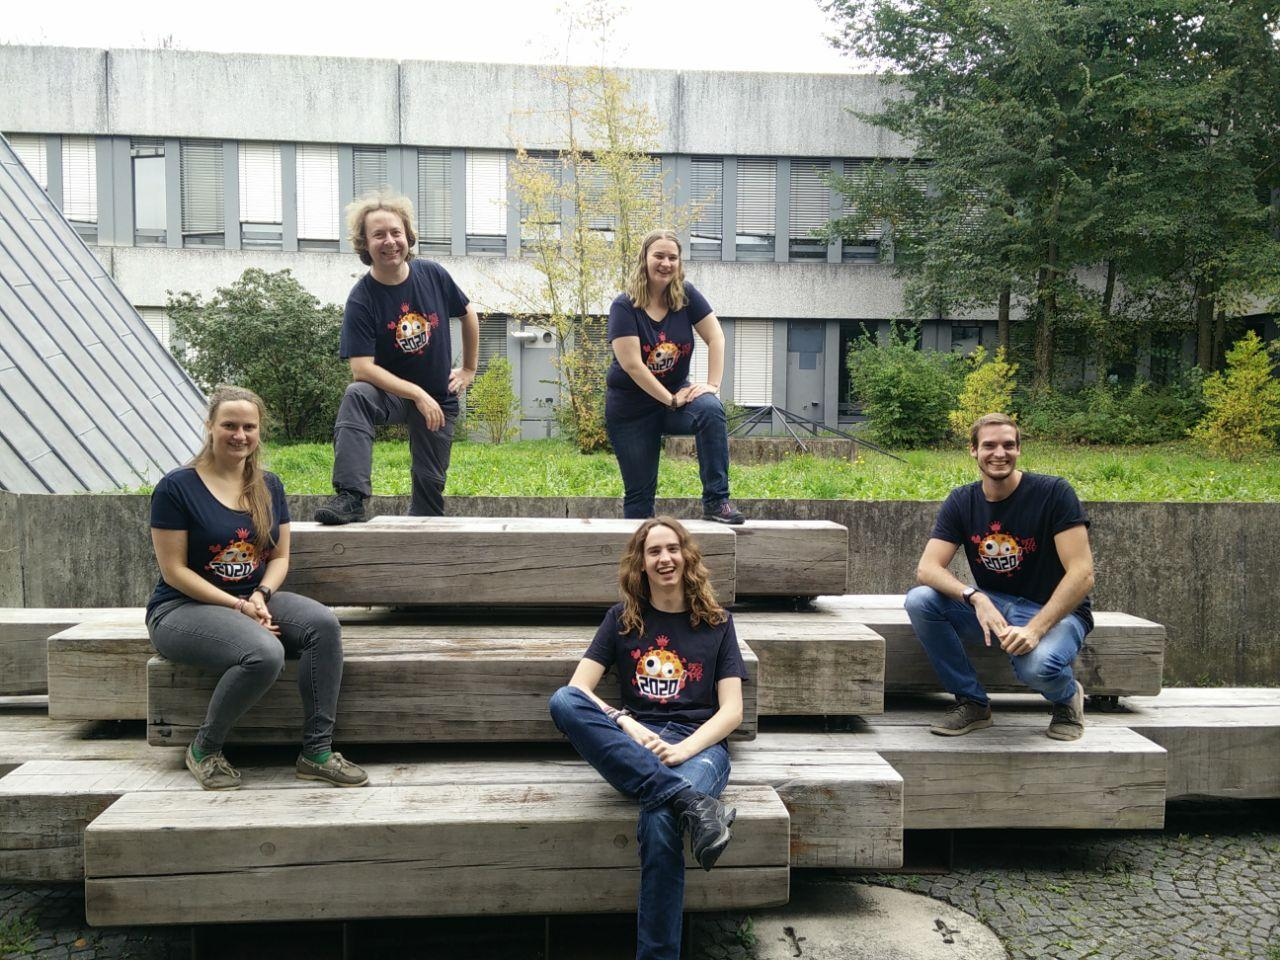
\includegraphics[width=.9\textwidth]{StAPF.jpg}
% \vspace{.5cm}
% \end{minipage}
% \begin{minipage}{.45\textwidth}
% Von links nach rechts:\\

% Sophie Pengers (Uni Köln)\\

% Leon Nutzinger (FU Berlin)\\

% Andreas Drotloff (Uni Würzburg)\\

% Maximilian Schneider (Uni Würzburg)\\

% Christoph Blattgerste (Uni Heidelberg)\\
% \end{minipage}
% \end{frame}

\begin{frame}{Was bisher geschah...}
 \begin{itemize}
  \item Resolutionen verschickt und veröffentlicht
  \begin{itemize}
    \item Resolution zur Novellierung des Bayrischen Hochschulgesetzes
    \item Forderungskatalog an eine BaFöG Novellierung
    \item Positionspapier zu FAIR und Open Data im Praktikum
    \item Positionspapier zu Vertrauenspersonen
    \item Positionspapier zum Solidarsemester-Bündnis
   \end{itemize}
   \item Unterstützung des Positionspapiers zum Qualitätsbericht systemakkreditierter Hochschulen 
 \end{itemize}
\end{frame}
%
%\begin{frame}{Ganz viele Diskussionen ...}
%  \begin{itemize}
%    \item Kommunikationswege der ZaPF
%    \item Planen neuer Workshops (Gewaltfreie Kommunikation, mentale Gesundheit, ...)
%    \item Austausch zu WissKomm ($\rightarrow$ siehe eigener Bericht)
%    \item Gespräch mit dem Wissenschaftsrat über studentische Beteiligung an Hochschulen
%    \item Kommende Orgas finden \& beraten
%    \item Koordinierung von Großprojekten (BaMa-Umfrage, Reformforum, Studienführer, ...)
%    \item Viele Kleinigkeiten ...
%  \end{itemize}
%\end{frame}

\begin{frame}{Beschlüsse des 19ten StAPF (OZaPFhiG bis Ostsee-ZaPF)}
  \begin{itemize}
      \item Wahl von Andreas zur STIMME der ZaPF
      \item Veröffentlichung der Broschüre zu stud. Engagement unter GNU GPLv3
      \item Mandatierung von Fabian Freyer zur Teilnahme an MODUS Auftaktveranstaltung der HRK
      \item Kommende ZaPF:
        \begin{itemize}
          \item Winter-ZaPF 2021/22: Fachschaft Göttingen
          \item Sommer-ZaPF 2022: Fachschaft Bochum (Muss das nicht im Endplenum erst offiziell gewählt werden?)
        \end{itemize}
  \end{itemize}
\end{frame}

%\begin{frame}
%  \begin{itemize}
%    \item ZaPF-Bericht verschickt und veröffentlicht
%    \item Evaluation aus Freiburg ausgewertet
%    \item 10 Sitzungen seit der ZaPF in Freiburg
%    \item Klausurtagung vom 6.-8.12.19 in Rostock zur Nachbereitung von Freiburg
%    \item Klausurtagung vom 24.-26.04.20 auf Balkonien zur Vorbereitung der Digital ZaPF
%    \item Planung der Digital-ZaPF nach der Absage aus Rostock
%  \end{itemize}
%  \vspace{5mm}
%  \begin{center}
%    \Large DANKE an alle, die uns dabei unterstützt haben!
%  \end{center}
%\end{frame}

\begin{frame}{Und sonst so?}
  \begin{itemize}
    \item 6 Sitzungen seit Ende der OZaPFhig
    \item Umsetzung der Briefwahlergebnisse der OZaPFhig
    \item Neustrukturierung des Wikis (unsere Arbeitsplattform)
    \item Vorstellung unserer Positionen auf der DPG Didaktiktagung
    \item Beratungen über Hygienekonzepte der Winter-ZaPF \& Klausurtagung
  \end{itemize}
\end{frame}

\begin{frame}{Akkreditierungspool}
    \begin{itemize}
        \item Der studentische Akkreditierungspool
        \begin{itemize}
        	\item sorgt für die Einflussnahme von Studierenden in Akkreditierungsverfahren
        	\item entsendet Studierendenvertreter in den Akkreditierungsrat und in Agenturgremien
        	\item vertritt studentische Interessen gegenüber Agenturen und anderen Stakeholdern
        \end{itemize}         
        \item Studierende erhalten anfangs eine Schulung in zweitägigen Seminaren
        \item Letzte Poolvernetzungstreffen: Dezember \& Januar
        \vspace{0.5cm}
        % PJ FIXME: Das stimmt nicht mehr (-;
        %\item Momentan keine Physiker im Systemakkreditierungspool
        \item[$\rightarrow$] Bei Interesse: Besucht den Akkreditierungs-Workshop für Einsteiger
    \end{itemize}
\end{frame}


\section{TOPF}

\begin{frame}{Was ist der TOPF?}
  \begin{minipage}{.5\textwidth}
    \begin{itemize}
      \item 2 DECkEL \footnotemark[1]
      \begin{itemize}
        \item Sean Bonkwoski (Bonn)
        \item Timo Prinz (Berlin, TU)
      \end{itemize}
      \item Viele HENkeL\footnotemark[2]\footnotemark[3]
      \item Server
      \item ... und ganz viele Dienste
    \end{itemize}
  \end{minipage}
  \hfill
  \begin{minipage}{.48\textwidth}
    \begin{minipage}[c]{.5\textwidth}
      
\includegraphics[height=.4\textheight]{sean.jpg}
      \captionof*{figure}{Sean}
    \end{minipage}
    \begin{minipage}[c]{.48\textwidth}
      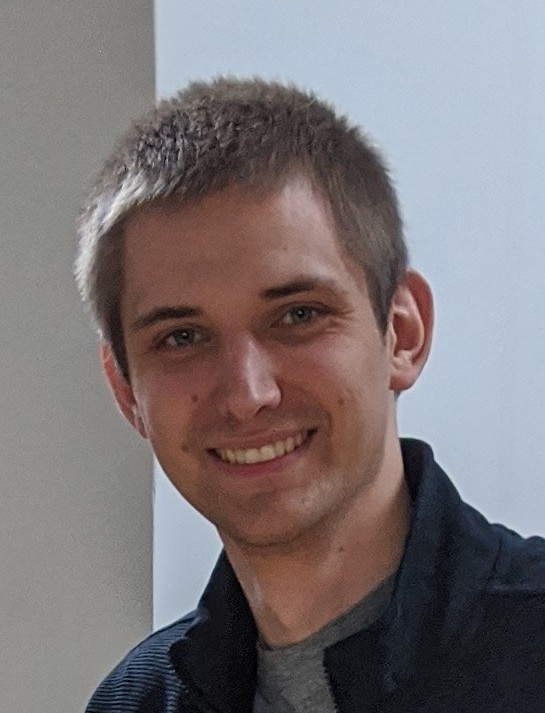
\includegraphics[height=.4\textheight]{timo.jpg}
      \captionof*{figure}{Timo}
    \end{minipage}
  \end{minipage}
  \footnotetext[1]{Dokumentations-, Einrichtungs- und Clusterfuckkoordinierende für EDV-Lösungen} 
  \footnotetext[2]{Helfende mit EDV- und Netzwerkkompetenzen für ergebnisorentierte Lösungen}
  \footnotetext[3]{Können gerne mehr werden ;-)}
\end{frame}

\section{KomGrem}

\begin{frame}\frametitle{KomGrem - Wer sind wir?}
 \begin{figure}
		\begin{subfigure}[t]{0.24\textwidth}
			
\includegraphics[width = \textwidth]{brunner.jpg}
			\caption*{Jacob Brunner (Augsburg)}
		\end{subfigure}
			\begin{subfigure}[t]{0.24\textwidth}
				
\includegraphics[width = \textwidth]{blaensdorf.jpg}
				\caption*{Sebastian Blänsdorf (Heidelberg)}
		\end{subfigure}
			\begin{subfigure}[t]{0.24\textwidth}
				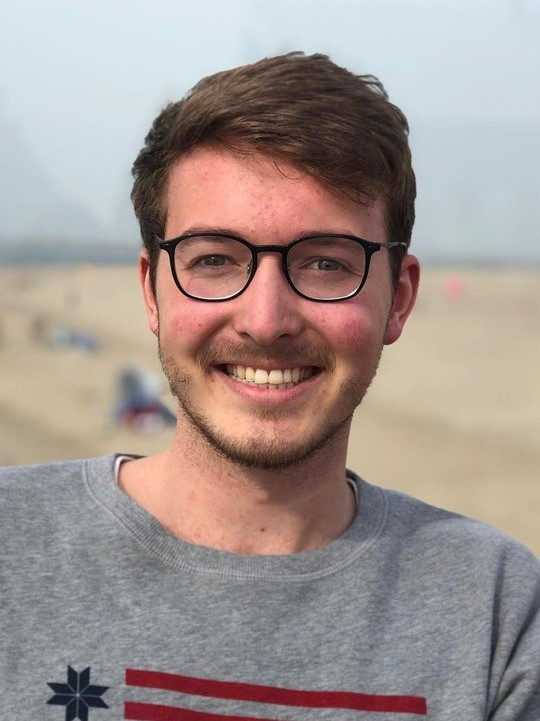
\includegraphics[width = \textwidth]{Nitschke.jpeg}
				\caption*{Jonah Nitschke (jDPG RG Dortmund)}
		\end{subfigure}
				\begin{subfigure}[t]{0.24\textwidth}
				\includegraphics[width = \textwidth]{boushmelev.jpg}
				\caption*{Anastasia Boushmelev (jDPG RG Siegen)}
		\end{subfigure}
 \end{figure}
\end{frame}

\begin{frame}\frametitle{KomGrem - Was machen wir?}
	\begin{block}{Was wir machen}
		\begin{itemize}
			\item Koordinierung der Zusammenarbeit von jDPG und ZaPF
			\item Austausch über mögliche Kooperationen bei verschiedenen Themen (CHE, Nachhaltigkeit etc.)
			\item Teilnahme an der KFP (Konferenz der Fachbereiche Physik)
			\item Verbesserung der Vernetzung zwischen Fachschaften und jDPG Regionalgruppen
		\end{itemize}
	\end{block}
\end{frame}

\subsection{NFDI-Beteiligung}
\begin{frame}{\insertsubsection}
	\vspace{-3mm}
	\begin{block}{Was ist NFDI und warum l"asst es mich nicht in Ruhe?}
		\begin{itemize}
			\item Nationale Forschundsdateninfrastruktur
			\item Etablierung einer technischen Infrastruktur zum Forschungsdatenmanagement
			\item FAIR-Prinzipien: Findabile, Accessible, Interoperable, Reusable
			\item \glqq Das O in FAIR\grqq: Open Data
		\end{itemize}
	\end{block}
	\pause
	\vspace{4mm}
	\scriptsize
	Beauftragte Personen:
	\begin{itemize}
		\item Merten Dahlkemper (Alumni, G"ottingen, CERN, jDPG)
		\item Janice Bode (M"unster)
		\item Philipp Jaeger (Alumni, Manitoba, Wuppertal, jDPG)
	\end{itemize}
\end{frame}

\begin{frame}{\insertsubsection}
	Ziele von ZaPF und jDPG
	\begin{itemize}
		\item Ber"ucksichtigung studentischer Interessen beim Aufbau der NFDI(s)
		\item ZaPF e.V. soll ``participant'' in NFDI4Phys - TA Data Literacy werden
		\item Darstellung unserer Ziele auf der Homepage von NFDI4Phys
		\item Zusammenarbeit mit FAIRmat, PUNCH4NFDI, (und DAPhNE) 
		\item Gemeinsames Panel Lehre@NFDI mit DPG, KFP, 3+1 Konsortien
		\vspace{4mm}\item[$\rightarrow$] Bei Interesse: Zum AK kommen!
	\end{itemize}
\end{frame}

\section{ZaPF e.V.}

\begin{frame}{Was tut der ZaPF e.V.?}
  \begin{block}{Aufgaben des e.V.}
    \begin{itemize}
      \item Strukturelle Unterstützung der ZaPF
      \item Infrastruktur
      \item Finanzielle Absicherung
      \item Rechtliche Absicherung
      \item Finanzierung für Gremien (z.B. Reisekosten)
      \item Unterstützung von Finanzschwachen Fachschaften
    \end{itemize}
  \end{block}
\end{frame}
  
\begin{frame}{Wer tut da was im ZaPF e.V.?}
  \begin{block}{Aktuelle Vorstände}
    \begin{minipage}{0.5\textwidth}
      \begin{figure}
      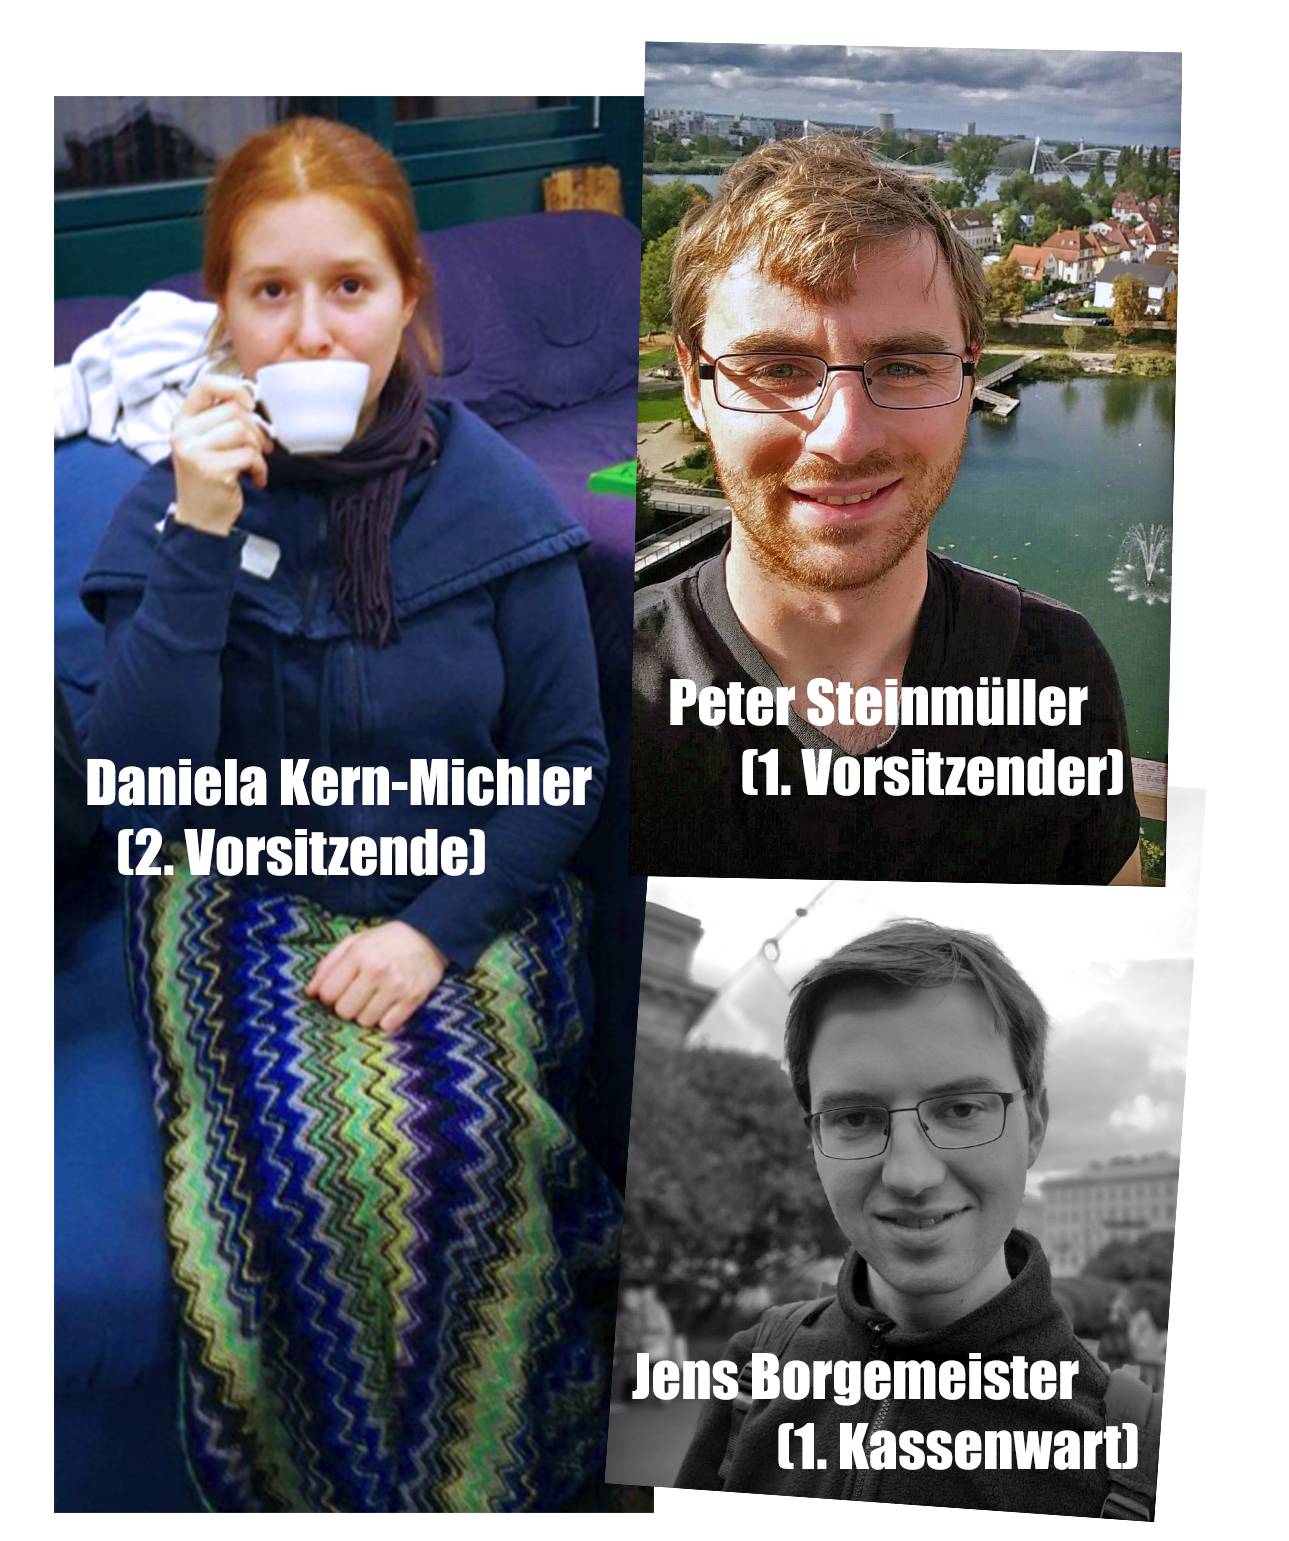
\includegraphics[height=.75\textheight]{ZapfeV.png}
      \end{figure}
    \end{minipage}
    \begin{minipage}{0.45\textwidth}
      \begin{itemize}
        \item Marcus Mikorski \mbox{(2. Kassenwart)}
        \item Fabian Freyer (IT)
        \item Lisa Dietrich (Finanzschwache Fachschaften)
        \item Marcel Nitsch (Bonn)
        \item Timo Rachel (Freiburg)
        \item Lena Wunderl (München)
        \item Richard Altenkirch (Rostock)
      \end{itemize}
    \end{minipage}
  \end{block}
\end{frame}
  
\begin{frame}{Was kann man tun im ZaPF e.V.?}
  \begin{block}{Fördermitglied werden}
    \begin{itemize}
    \item Fördermitglieder sind natürliche Personen (z.B. du) oder juristische (euer Fachschaft oder Verein)
    \item Ihr unterstützt den Verein mit Mitgliederbeiträgen
    \end{itemize}
  \end{block}
  \begin{block}{Mitglied werden}
    \begin{itemize}
    \item Normale Mitglieder entscheiden über die Tätigkeiten des Vereins
    \item Diese zahlen keinen Beitrag
    \end{itemize}
  \end{block}
\end{frame}
  
\begin{frame}{Mitgliederversammlung am 12.11. um 19 Uhr}
  \begin{block}{Tagesordnung}
    \begin{multicols}{2}
      \begin{enumerate}\small
        \item Feststellung der Tagesordnung
        \item Wahl des Protokollführers
        \item Wahl der Versammlungsleitung
        \item Feststellung der Beschlussfähigkeit
        \item Genehmigung der letzten Protokolle
        \item Bericht des Vorstands
        \item Bericht des Kassenprüfers
        \item Umgang mit Corona Situtation
        \item Sonstiges
      \end{enumerate}
    \end{multicols}
  \end{block}
  \begin{block}{Ort}
    Die MV findet Online statt. Der Link dazu wird in den kommenden Tage im ZaPF-Wiki (\url{https://zapf.wiki/WiSe20_MV_ZaPFeV}) veröffentlicht.
  \end{block}
\end{frame}

\begin{frame}{Mitgliederversammlung am 12.11. um 19 Uhr}
  \begin{block}{Corona Situation}
    Die MV wird rein informell sein.\\
    Personenwahlen sind (aktuell) nicht online möglich.\\
    Der Vorstand bleibt, entsprechend dem Corona-Gesetz, bis zur nächsten Wahl bestehen.\\[1.5em]
    Nach der ZaPF soll es eine MV für Neuwahlen geben, welche dann in Person stattfinden soll.
  \end{block}
\end{frame}

\begin{frame}{Kommende ZaPFen}
  \begin{itemize}
    % \vspace{05cm}
    \item Wintersemester 2021 in Göttingen
    \item Sommersemester 2022 ...
    \item Wintersemester 2022 \textit{\color{blue}{bei euch?}}    
\end{itemize}
    \vspace{1cm}
    \begin{center}
      \huge \textbf{Tosenden Applaus für die ausrichtenden Orgas!}
    \end{center}
\end{frame}

\begin{frame}[plain]
  \begin{center}
    \Huge Habt ihr Fragen an uns?
    \end{center}
\end{frame}


\section{Wissenschaftskommunikation}

\end{document}
